\documentclass[12pt, a4paper]{article}

% --- PACOTES FUNDAMENTAIS ---
\usepackage[utf8]{inputenc}
\usepackage[T1]{fontenc}
\usepackage[brazil]{babel}
\usepackage{helvet}
\renewcommand{\familydefault}{\sfdefault} % Fonte Arial/Helvetica
\usepackage{amsmath} % Fórmulas matemáticas
\usepackage{graphicx} % Inserção de imagens
\usepackage{enumitem} % Listas customizadas
\usepackage{indentfirst} % Indenta o primeiro parágrafo (Padrão ABNT)
\usepackage{setspace} % Espaçamento entrelinhas
\usepackage{xurl} % Quebra de linha em URLs
\usepackage[hidelinks]{hyperref} % Links clicáveis sem caixas
\urlstyle{same}

% --- CONFIGURAÇÃO DE MARGENS E CABEÇALHO ---
\usepackage[a4paper, top=4cm, headheight=2.5cm, bottom=2cm, left=3cm, right=2cm]{geometry}
\usepackage{fancyhdr}

\pagestyle{fancy}
\fancyhf{} 
\renewcommand{\headrulewidth}{0pt}
% Logotipo/cabeçalho da FICE
\chead{\noindent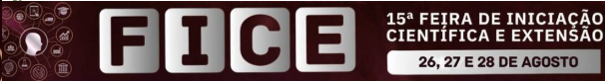
\includegraphics[width=\textwidth]{Imagem1.png}}

% --- ESPAÇAMENTO DAS NOTAS DE RODAPÉ ---
\setlength{\skip\footins}{1.5cm} 

% --- ATALHO DE FORMATAÇÃO DAS SEÇÕES ---
\newcommand{\titlesection}[1]{
    \vspace{1.5em}
    \noindent\textbf{\MakeUppercase{#1}}
    \vspace{1em}\par
}

\begin{document}
\onehalfspacing

% --- TÍTULO E AUTORES ---
\begin{center}
    \textbf{TÍTULO DO TRABALHO: Subtítulo (se houver)}
    
    \vspace{1.5em}
    Nome do Autor 1$^{1}$; Nome do Autor 2$^{2}$; Nome do Autor 3$^{3}$; Nome do Orientador$^{4}$
\end{center}

% Notas de rodapé com afiliações (Já configurado para Ciência da Computação no IFC)
\footnotetext[1]{Estudante do curso de Ciência da Computação. Instituto Federal Catarinense (IFC) - Campus Videira. E-mail: autor1@email.com}
\footnotetext[2]{Estudante do curso de Ciência da Computação. Instituto Federal Catarinense (IFC) - Campus Videira. E-mail: autor2@email.com}
\footnotetext[3]{Estudante do curso de Ciência da Computação. Instituto Federal Catarinense (IFC) - Campus Videira. E-mail: autor3@email.com}
\footnotetext[4]{Professor Orientador. Instituto Federal Catarinense (IFC) - Campus Videira. E-mail: orientador@ifc.edu.br}

% --- INTRODUÇÃO ---
\titlesection{INTRODUÇÃO}
[Insira aqui a introdução do seu projeto. Exponha o assunto, informe a delimitação, os objetivos e as justificativas que levaram à escolha do tema para demonstrar a relevância do estudo.]

% --- PROCEDIMENTOS METODOLÓGICOS ---
\titlesection{PROCEDIMENTOS METODOLÓGICOS (materiais e métodos)}

[Descreva como o projeto será executado. Pode utilizar a listagem sugerida pelo modelo:]

\begin{enumerate}[label=\alph*)]
    \item Início e término da implementação do projeto: [Período planejado].
    \item Local onde será desenvolvido o trabalho: Instituto Federal Catarinense (IFC) - Campus Videira.
    \item População envolvida: [Público-alvo].
    \item Instrumentos utilizados: [Softwares, hardwares, questionários, etc.].
    \item Procedimentos: [Descrição das etapas e técnicas de desenvolvimento].
    \item Métodos de análise dos dados: [Como os resultados serão avaliados].
\end{enumerate}

% --- PLANO DE ATIVIDADES ---
\titlesection{PLANO DE ATIVIDADES}
[Insira aqui o cronograma do projeto. É comum utilizar uma tabela ou lista de meses indicando o que será feito (ex: levantamento bibliográfico, desenvolvimento do backend, testes de software, escrita do relatório).]

% --- ORÇAMENTO ---
\titlesection{ORÇAMENTO}
[Descreva os custos previstos para a execução do projeto. Pode incluir infraestrutura em nuvem, aquisição de componentes de hardware, licenças de software ou materiais de consumo. Caso não haja custos, especifique que serão utilizados os laboratórios e recursos já disponíveis na instituição.]

% --- REFERÊNCIAS ---
\begin{center}
    \vspace{1.5em}
    \textbf{REFERÊNCIAS}
    \vspace{1em}
\end{center}

\begin{singlespace}
\noindent SOBRENOME, Nome do Autor. \textbf{Título do livro ou artigo em negrito}. Edição. Cidade: Editora, Ano.

\vspace{1em}
\noindent SOBRENOME, Nome do Autor 2. Título do artigo. \textbf{Nome da Revista em negrito}, Cidade, v. 1, n. 1, p. 1-10, Ano.
\end{singlespace}

\end{document}